\chapter{C-RAN for LoRa}
\label{chap:cran_for_lora}

\section{Goal}
The goal is to set up a minimal working environment for a LoRa C-RAN.
The gateway's functionality should separated into an RRH and BBU component and the 
BBU component should be virtualized and run on general purpose hardware. 
A simple network server should process the uplink message and schedule a response if required. From this setup 
basic network requirements can be derived and measured as well as costs estimated.

\section{Methods}

\begin{figure}
    \centering
    \begin{subfigure}[b]{0.25\textwidth}
     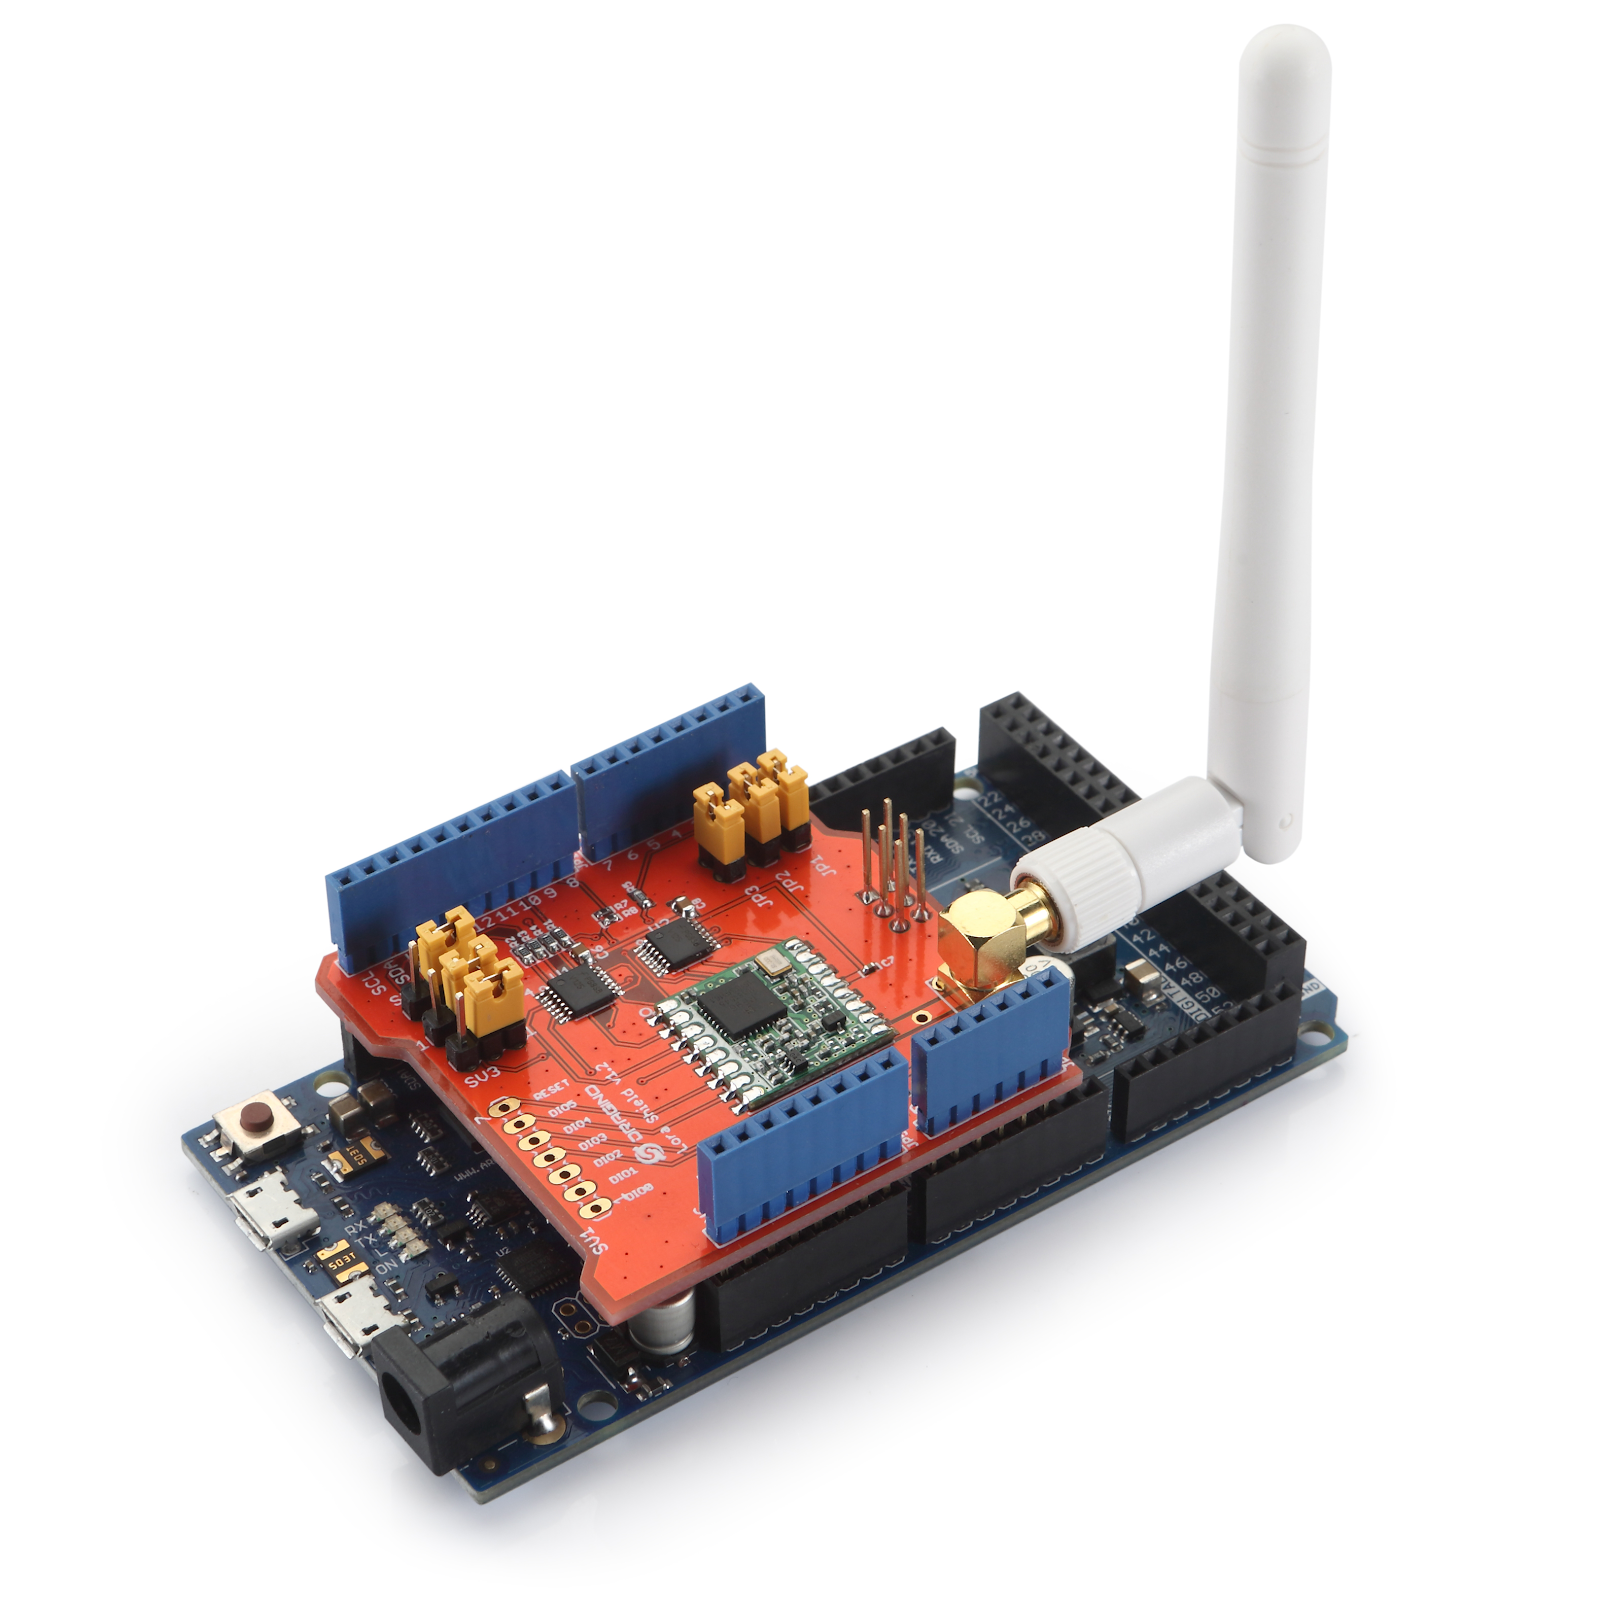
\includegraphics[width=1\textwidth]{figures/arduino.png}
     \caption{Arduino with LoRa shield}
    \end{subfigure}%
    \hspace{2em}
    \begin{subfigure}[b]{0.25\textwidth}
     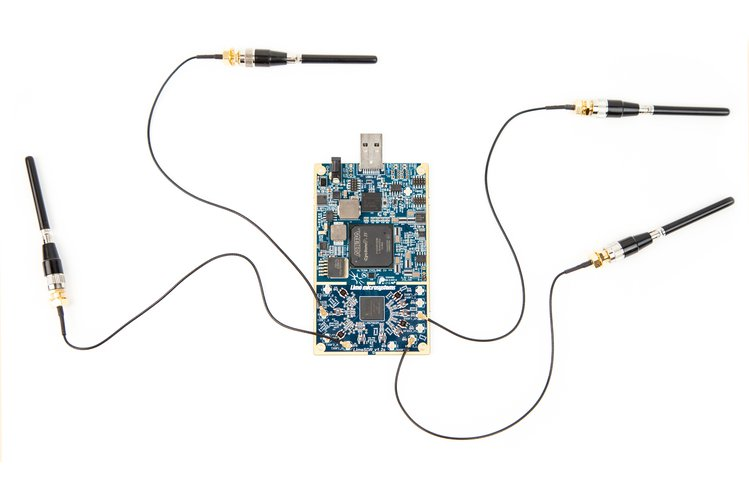
\includegraphics[width=1\textwidth]{figures/limesdr.png}
     \caption{LimeSDR mini}
    \end{subfigure}
    \hspace{2em}
    \begin{subfigure}[b]{0.25\textwidth}
     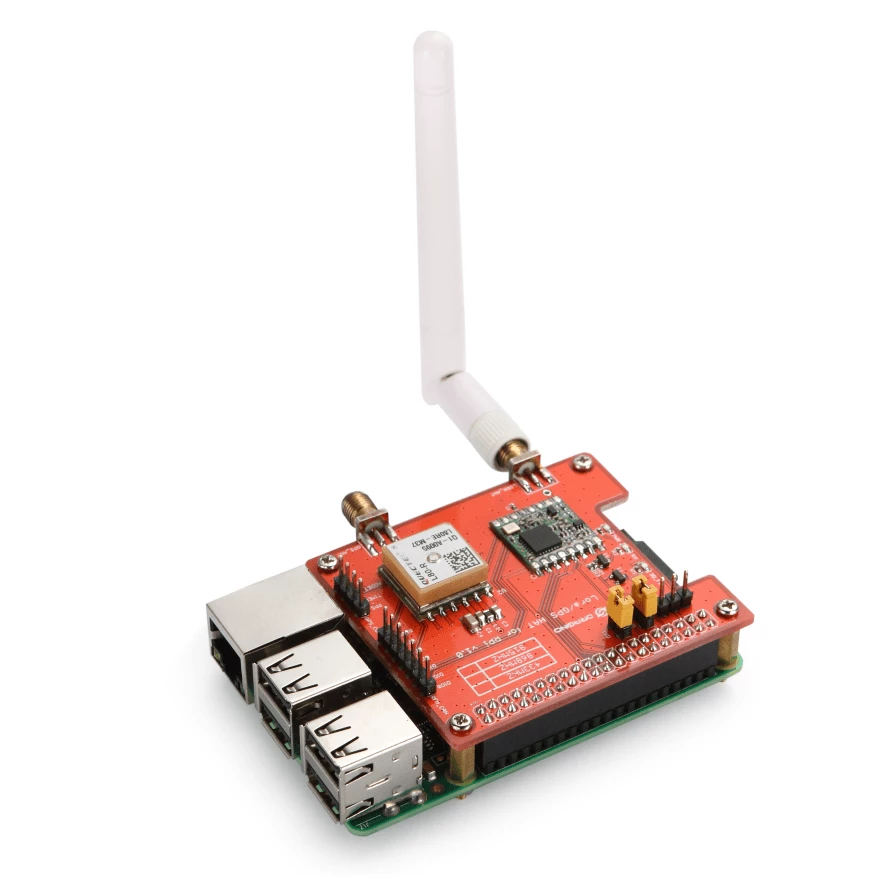
\includegraphics[width=1\textwidth]{figures/raspberry.png}
     \caption{Raspberry Pi with LoRa hat}
    \end{subfigure}
    \caption{Hardware devices}
   \end{figure}
\subsection{Sending uplink signals}
Uplink signals are sent with an arduino device equipped with a LoRa shield. 
The arduino is controlled with an adapted form of the IBM LoraMAC-in-C (LMIC) library, modified to run on arduino devices.
Using this library we implemented a simple communication protocol where a queue of packets is sent out in an interval.
See section~\ref{sec:comm_prot} for detailed information.
% \url{https://github.com/matthijskooijman/arduino-lmic}.
\subsection{RRH and BBU}
For splitting up the LoRa gateway's functionality we use two laptops. 
One laptop has the LimeSDR mini plugged in and serves as the RRH. The other decodes the LoRa
signal in software, processes the signal and also generates LoRa signals in software and sends those downlink I/Q samples back to the RRH.
The processes on the second laptop run in virtualized environment with docker, more specifically docker compose, dockers orchestration tool.
\\
The LoRa OOT module by Robyns et al. has a branch called "encoder" where they began the implementation of modulating an uplink LoRa signal in software.
It is able to generate a specific test packet but the modulated signal has errors as we saw when we inspected the data payload on the LoRa gateway.
Having an uplink signal generator was a nice starting point, but we needed something to generate downlink signal. In the end we extended the existing implementation
by adding a downlink signal generation ability, see section~\ref{todo}.
\\
Though, as a first workaround we set up a private LoRaWAN network, scheduled a downlink, and recorded it to a file. Now we can stream that file as a response by streaming its content,
which are I/Q samples, to the RRH.


\subsection{Network tools}
For measuring network traffic, the tool "bmon" is used which stands for bandwidth monitor.
It estimates the bits per second on all available network interfaces, ingoing as well as outgoing. 
For adding network delay we used the tool "netem" which stands for network emulator. With netem we can add a delay to the qdisc scheduler
which controls the processing the IP packets sent over the ethernet network interface.
Both tools can easily be install with the "apt" package manager for ubuntu.
\newpage
% getting a downlink signal
% recording from thethingsnetwrok
% recording from private networks
% manipualting private gateway
% offline generation of downlink signal see chapter



\section{Architecture}
This section aims to first give a high level overview of the architecture and then give a more detailed 
architectural overview of each component.
Figure~\ref{fig:high_level_arch} shows the high level architecture with all the hardware components involved.
There are two laptops in the same network connected by an ethernet cable. One laptop serves as an RRH. It has the LimeSDR mini 
plugged into its USB port so it can send and receive signals.
\begin{figure}[h]
    \centering
    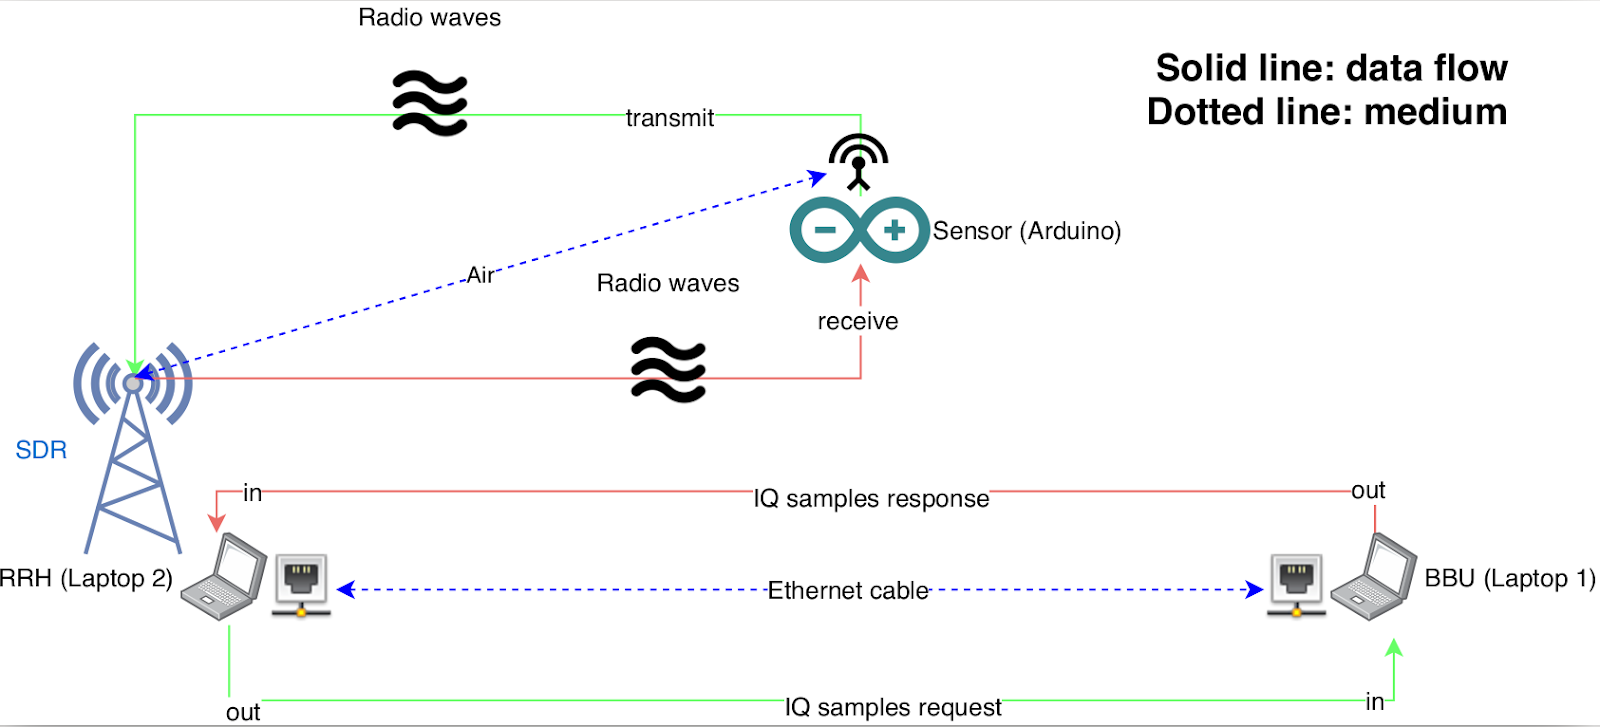
\includegraphics[width=1\textwidth]{figures/high_level_arch.png}
    \caption{High level architecture}
    \label{fig:high_level_arch}
\end{figure}
Incoming signals come from the arduino device. The arduino transmits packets over the air as radio waves. Those get picked up 
by the RRH which converts the analog signal and send them as digital 32bit floats as I/Q samples over ethernet to the second laptop.
This second laptop is the host for the virtual BBU that runs in a docker container. There the signals get demodulated and decoded.
Then the decoded signal gets processed. In case a response is requested, a response signal is generated and sent as I/Q samples back to the RRH.
From the it gets transmitted back to the arduino.
\subsection{RRH and BBU}
The RRH is the simplest component. It has an antenna for input and one for output. In Figure~\ref{fig:seq_diagram} the RRH is composed by the two 
components "SDR RX" and "SDR TX". They correspond to the physical RX and TX slots ond the SDR device. The BBU is the "Lora Decoder" component. It runs 
in a virtualized environment. Decoded messages get passed to the "Python Script" component. This acts as a network server that schedules an acknowledgement
message back to the arduino. It could run on a third laptop connected via ethernet to the BBU laptop, but for our purposes it runs on the same laptop
as the BBU but in a separate docker container.
\begin{figure}[h]
    \centering
    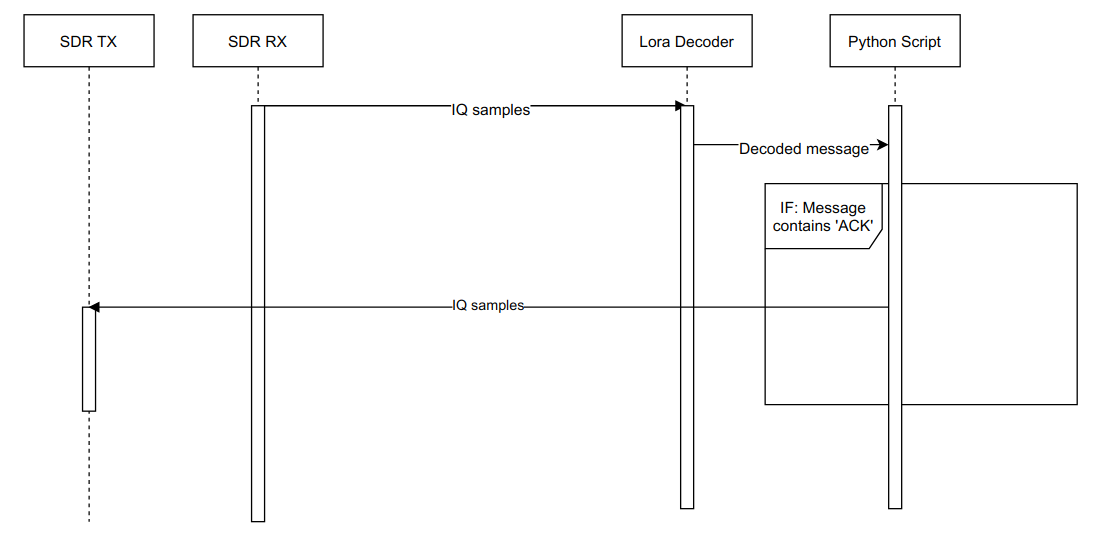
\includegraphics[width=1\textwidth]{figures/seq_diagram.png}
    \caption{Sequence diagram}
    \label{fig:seq_diagram}
\end{figure}


\section{Implementation}
All communication between the components happens over sockets. We use the ZeroMQ (ZMQ) networking library.
It is a good messaging library that offers N-to-N patterns as possible ways to connect the sockets, such as a request-reply pattern
or pub-sub pattern and many more~\cite{zeromq}.
GNU Radio offers ZMQ blocks out of the box, The TCP sink and source blocks for socket communication are still available but deprecated. 
For communication between the RRH and the BBU the pub-sub (publish-subscribe) pattern is used.
Figure~\ref{fig:seq_diagram} shows the "PUB" and "SUB" blocks and the data flow.
The RRH has a PUB sockets that takes as input the I/Q sample stream generated by the RX of the SDR.
The SUB socket in the BBU subscribes to this publishing socket. As this socket connection happens with TCP, the I/Q samples arrive in the order
they are sent an can be directly passed to the LoRa Decoder. Robyns' et al. implementation of LoRa Decoder sends the decoded message 
out on a UDP socket.  The "Python Script" block which is our LoRa network server takes the decoded messages over on this UDP socket and then, streams out 
I/Q samples of the response message over a ZMQ publishing socket to which the RRH's TX slot subscribes to. This closes the cycle.
One of the advantages of using ZMQ is that the sockets can be given the option to not time out or close. This means a subscribing socket 
can be started before a publishing socket without issues. The subscribing socket can wait for the publishing socket to get instantiated. For our architecture 
this means the docker containers for the RRH and BBU can be started in any order and more instances of the BBU can be added at runtime. The sub-pub pattern 
allows new subscribers and publisher to join.

\begin{figure}[h]
    \centering
    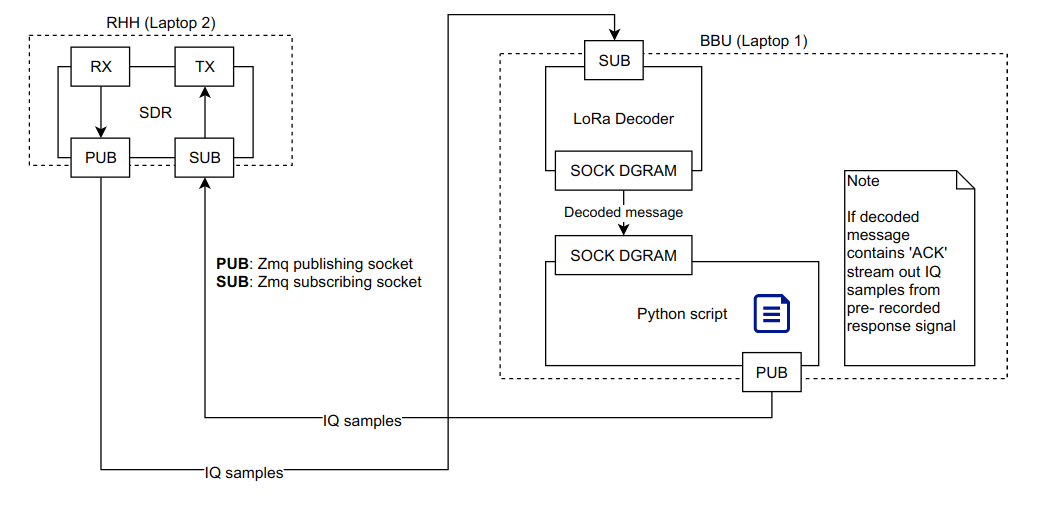
\includegraphics[width=1\textwidth]{figures/impl_diagram.png}
    \caption{Socket communication between components}
    \label{fig:impl_diagram}
\end{figure}

\subsection{RRH}
The RRH implementation is straightforward. Figure~\ref{fig:RRH_impl} show the necessary 
GNU Radio blocks. On the left is the RX block of the LimeSDR that streams the incoming signals to the 
PUB socket. The response message from the networks server to send out comes through a SUB socket which 
streams directly to the TX block of the LimeSDR on the far right of the Figure.
The parameter blocks allow the passing of command line arguments to the resulting application to configure
the socket addresses if necessary. As there is a OOT module needed for GNU Radio to work with the LimeSDR, a the 
RRH comes also in a docker container to quickly get started as the necessary dependencies have all been installed
in that container.
\begin{figure}[h]
    \centering
    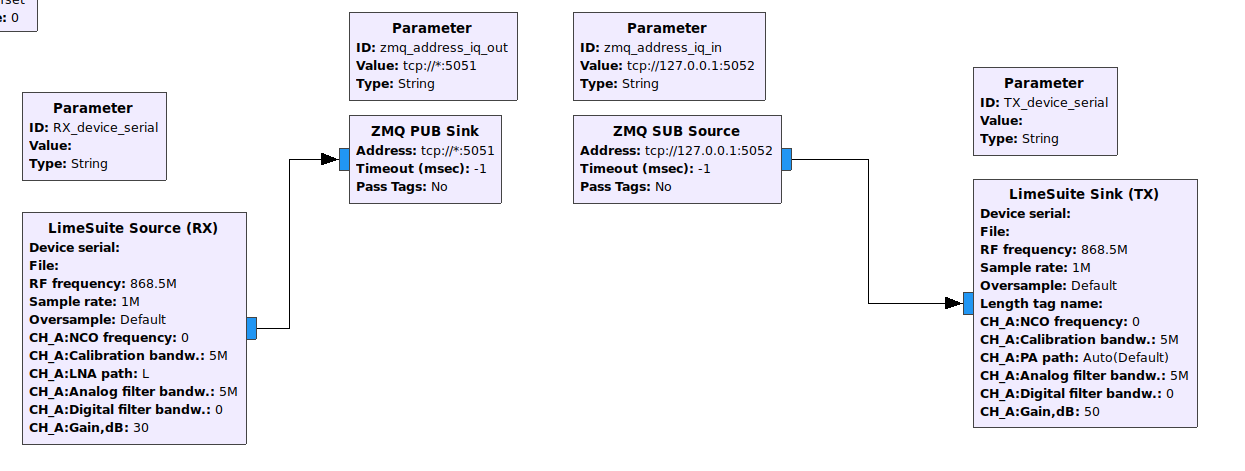
\includegraphics[width=1\textwidth]{figures/RRH_impl.png}
    \caption{GNU Radio blocks for the RRH}
    \label{fig:RRH_impl}
\end{figure}

\subsection{BBU}
The BBU as shown in Figure~\ref{fig:BBU_impl} takes in the RX stream of the RRH on a SUB socket,
passes the I/Q samples to the LoRa decoder. The decoder decodes LoRa signal and outputs them as a 
message on the message socket sink, far right in the Figure.


\begin{figure}[h]
    \centering
    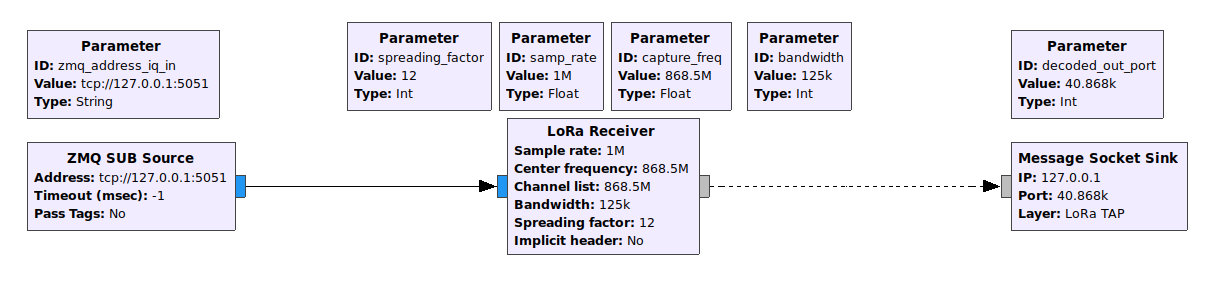
\includegraphics[width=1\textwidth]{figures/BBU_impl.png}
    \caption{GNU Radio blocks for the BBU}
    \label{fig:BBU_impl}
\end{figure}

The python script which acts as our network server, inspects the message payload and if an 
acknowledgement is required by the sender it generates the response signal. 
Listing~\ref{lst:python_code} shows an excerpt of that python script.
The acknowledgement message is a recording of a LoRa downlink signal. Its I/Q samples get read into memory.
The script connects to the UDP socket. As the BBU component and this python script run on the same host, it connects
to 127.0.0.1, the port is passed as argument to the script. As the focus lies on the split between RRH and BBU we decided
to hard code the IP address to localhost for the LoRa decoder and the network server as they run on the same machine as depicted 
in Figure~\ref{fig:impl_diagram}. 
Then, in an endless loop, data gets received from the socket. The buffer size is 1024 bytes.
Whenever "ACK" is in the message payload, the acknowledgement signal get streamed out over a ZMQ publishing socket.
\\
The BBU and the network server run each in a container started with docker compose.


\begin{listing}[H]
\begin{minted}[frame=single,linenos=false]{python}
import zmq
import socket
...
with open (dir_path + "/ACK_DOWN_SF12_CR4.raw") as f:
    ack = f.read()
...
zmq_socket = context.socket(zmq.PUB)
...
s = socket.socket(socket.AF_INET, socket.SOCK_DGRAM)
s.bind(("127.0.0.1", udp_port))
print ('listen for decoded lora packages on udp port ' + str(udp_port))
while True:
    data, addr = s.recvfrom(1024)

    if ("ACK" in data):
        zmq_socket.send(ack) 
    else:
        print ("received package requests no ACK")
     
    
    \end{minted}
    \caption{Excerpt of the python script that functions as the network server}
    \label{lst:python_code}
\end{listing}

\subsection{Communication Protocol Arduino}
\label{sec:comm_prot}

The LMIC library runs a loop that executes jobs scheduled to run at a specified time. 
In the \emph{setup()} function that runs once when the arduino starts settings such as 
the spreading factor, frequency and coding rate are set. Also, the initial job for the LMIC is initialized there, see 
Listing~\ref{lst::ard_setup} last line.

\begin{listing}[H]
    \begin{minted}[frame=single]{c++}
void setup() {
  Serial.begin(9600);
  ...
  // initialize runtime env
  os_init();
  ...
  // Set up these settings once, and use them for both TX and RX
  LMIC.freq = 868500000;
  LMIC.txpow = 27; // Maximum TX power
  LMIC.datarate = DR_SF12;
  // This sets CR 4/5, BW125 (except for DR_SF7B, which uses BW250)
  LMIC.rps = updr2rps(LMIC.datarate);

  Serial.println("Started");
  Serial.flush();

  // setup initial job
  os_setCallback(&txjob, my_tx_func);
}
    \end{minted}
    \caption{Arduino setup() function}
    \label{lst::ard_setup}
    
\end{listing}

The last line schedules the initial job  \emph{txjob} with the \emph{my\_tx\_func} function that gets run
on execution of the job.


\begin{listing}[H]
    \begin{minted}[frame=single]{c++}
static void my_tx_func(osjob_t *job) {
if (currentPacketIndex < numOfPackets) {
    char lastThree[3];
    memcpy(lastThree, &myPackets[currentPacketIndex][length - 3], 3);
    const char ack[] = {'A', 'C', 'K'};
    if (!memcmp(lastThree, ack, 3)) {
        // send and start rx for receiving ACK
        Serial.print("transmitting packet with ACK, packet: ");
        tx(myPackets[currentPacketIndex], my_txdone_func);
    } else {
        // send and schedule next packet
        Serial.print("transmitting packet without ACK, packet: ");
        tx(myPackets[currentPacketIndex], my_txdone_no_ack_func);
    }
    os_setTimedCallback(&txjob, os_getTime() +
                            ms2osticks(TX_INTERVAL), my_tx_func);
    } else {
        Serial.println("No more packets to send, done");
    }
}
    \end{minted}
    \caption{\emph{my\_tx\_fun} function}
    \label{lst::ard_mytx}
    
\end{listing}



\section{Results}

\chapter{LoRa Tools}

